\documentclass[10pt,landscape,a4paper]{article}
%\usepackage[utf8]{inputenc}
%\usepackage[ngerman]{babel}
\usepackage[normalem]{ulem}
\usepackage{tikz}
\usetikzlibrary{shapes,positioning,arrows,fit,calc,graphs,graphs.standard}
\usepackage[nosf]{kpfonts}
\usepackage[t1]{sourcesanspro}
%\usepackage[lf]{MyriadPro}
%\usepackage[lf,minionint]{MinionPro}
\usepackage{bold-extra}
\usepackage{multicol}
\usepackage{wrapfig}
\usepackage[top=0mm,bottom=1mm,left=0mm,right=1mm]{geometry}
\usepackage[framemethod=tikz]{mdframed}
\usepackage{microtype}
%\usepackage{physics}
\usepackage{tabularx}
\usepackage{hhline}
\usepackage{makecell}
\usepackage{mathtools}

\usepackage{listings}

\DeclarePairedDelimiter{\ceil}{\lceil}{\rceil}

\newcommand\codeblue[1]{\textcolor{blue}{\code{#1}}}

\usepackage{lastpage}
\usepackage{datetime}
\yyyymmdddate
\renewcommand{\dateseparator}{-}
\let\bar\overline

\definecolor{myblue}{cmyk}{1,.72,0,.38}

\def\firstcircle{(0,0) circle (1.5cm)}
\def\secondcircle{(0:2cm) circle (1.5cm)}

\colorlet{circle edge}{myblue}
\colorlet{circle area}{myblue!5}

\tikzset{filled/.style={fill=circle area, draw=circle edge, thick},
outline/.style={draw=circle edge, thick}}

\pgfdeclarelayer{background}
\pgfsetlayers{background,main}

%\everymath\expandafter{\the\everymath \color{myblue}}
%\everydisplay\expandafter{\the\everydisplay \color{myblue}}


\renewcommand{\baselinestretch}{.8}
\pagestyle{empty}

\global\mdfdefinestyle{header}{%
  linecolor=gray,linewidth=1pt,%
  leftmargin=0mm,rightmargin=0mm,skipbelow=0mm,skipabove=0mm,
}

\newcommand{\header}{
  \begin{mdframed}[style=header]
    \footnotesize
    \sffamily
    CS3210 Midterms Cheatsheet v1.0 (\today)\\
    by~Julius Putra Tanu Setiaji,~page~\thepage~of~\pageref{LastPage}
  \end{mdframed}
}

\let\counterwithout\relax
\let\counterwithin\relax
\usepackage{chngcntr}

\usepackage{verbatim}

\usepackage{etoolbox}
\makeatletter
\preto{\@verbatim}{\topsep=0pt \partopsep=0pt }
\makeatother

\counterwithin*{equation}{section}
\counterwithin*{equation}{subsection}
\usepackage{enumitem}
\newlist{legal}{enumerate}{10}
\setlist[legal]{label*=\arabic*.,leftmargin=2.5mm}
\setlist[itemize]{leftmargin=3mm}
\setlist[enumerate]{leftmargin=3.5mm}
\setlist{nosep}
\usepackage{minted}

\def\code#1{\texttt{#1}}

\newenvironment{descitemize} % a mixture of description and itemize
{\begin{description}[leftmargin=*,before=\let\makelabel\descitemlabel]}
{\end{description}}

\newcommand{\descitemlabel}[1]{%
  \textbullet\ \textbf{#1}%
}
\makeatletter



\renewcommand{\section}{\@startsection{section}{1}{0mm}%
  {.2ex}%
  {.2ex}%x
{\color{myblue}\sffamily\small\bfseries}}
\renewcommand{\subsection}{\@startsection{subsection}{1}{0mm}%
  {.2ex}%
  {.2ex}%x
{\sffamily\bfseries}}
\renewcommand{\subsubsection}{\@startsection{subsubsection}{1}{0mm}%
  {.2ex}%
  {.2ex}%x
{\rmfamily\bfseries}}



\def\multi@column@out{%
  \ifnum\outputpenalty <-\@M
    \speci@ls \else
  \ifvoid\colbreak@box\else
    \mult@info\@ne{Re-adding forced
    break(s) for splitting}%
    \setbox\@cclv\vbox{%
      \unvbox\colbreak@box
    \penalty-\@Mv\unvbox\@cclv}%
  \fi
  \splittopskip\topskip
  \splitmaxdepth\maxdepth
  \dimen@\@colroom
  \divide\skip\footins\col@number
  \ifvoid\footins \else
    \leave@mult@footins
  \fi
  \let\ifshr@kingsaved\ifshr@king
    \ifvbox \@kludgeins
      \advance \dimen@ -\ht\@kludgeins
      \ifdim \wd\@kludgeins>\z@
        \shr@nkingtrue
      \fi
    \fi
    \process@cols\mult@gfirstbox{%
      %%%%% START CHANGE
      \ifnum\count@=\numexpr\mult@rightbox+2\relax
        \setbox\count@\vsplit\@cclv to \dimexpr \dimen@-1cm\relax
        \setbox\count@\vbox to \dimen@{\vbox to 1cm{\header}\unvbox\count@\vss}%
      \else
        \setbox\count@\vsplit\@cclv to \dimen@
      \fi
      %%%%% END CHANGE
      \set@keptmarks
      \setbox\count@
      \vbox to\dimen@
      {\unvbox\count@
        \remove@discardable@items
    \ifshr@nking\vfill\fi}%
    }%
    \setbox\mult@rightbox
    \vsplit\@cclv to\dimen@
    \set@keptmarks
    \setbox\mult@rightbox\vbox to\dimen@
    {\unvbox\mult@rightbox
      \remove@discardable@items
  \ifshr@nking\vfill\fi}%
    \let\ifshr@king\ifshr@kingsaved
  \ifvoid\@cclv \else
    \unvbox\@cclv
    \ifnum\outputpenalty=\@M
  \else
    \penalty\outputpenalty
  \fi
  \ifvoid\footins\else
    \PackageWarning{multicol}%
    {I moved some lines to
      the next page.\MessageBreak
      Footnotes on page
    \thepage\space might be wrong}%
  \fi
  \ifnum \c@tracingmulticols>\thr@@
\hrule\allowbreak \fi
  \fi
  \ifx\@empty\kept@firstmark
    \let\firstmark\kept@topmark
    \let\botmark\kept@topmark
  \else
    \let\firstmark\kept@firstmark
    \let\botmark\kept@botmark
  \fi
  \let\topmark\kept@topmark
  \mult@info\tw@
  {Use kept top mark:\MessageBreak
    \meaning\kept@topmark
    \MessageBreak
    Use kept first mark:\MessageBreak
    \meaning\kept@firstmark
    \MessageBreak
    Use kept bot mark:\MessageBreak
    \meaning\kept@botmark
    \MessageBreak
    Produce first mark:\MessageBreak
    \meaning\firstmark
    \MessageBreak
    Produce bot mark:\MessageBreak
    \meaning\botmark
  \@gobbletwo}%
  \setbox\@cclv\vbox{\unvbox\partial@page
  \page@sofar}%
  \@makecol\@outputpage
  \global\let\kept@topmark\botmark
  \global\let\kept@firstmark\@empty
  \global\let\kept@botmark\@empty
  \mult@info\tw@
  {(Re)Init top mark:\MessageBreak
    \meaning\kept@topmark
  \@gobbletwo}%
  \global\@colroom\@colht
  \global \@mparbottom \z@
  \process@deferreds
\@whilesw\if@fcolmade\fi{\@outputpage
    \global\@colroom\@colht
  \process@deferreds}%
  \mult@info\@ne
  {Colroom:\MessageBreak
    \the\@colht\space
    after float space removed
  = \the\@colroom \@gobble}%
  \set@mult@vsize \global
  \fi}
  \global\let\tikz@ensure@dollar@catcode=\relax

  \def\mathcolor#1#{\@mathcolor{#1}}
  \def\@mathcolor#1#2#3{%
    \protect\leavevmode
    \begingroup
    \color#1{#2}#3%
    \endgroup
  }

  \makeatother
  \setlength{\parindent}{0pt}

  \setminted{tabsize=2, breaklines}
  % Remove belowskip of minted
  \setlength\partopsep{-\topsep}


  \newcolumntype{a}{>{\hsize=1.5\hsize}X}
  \newcolumntype{b}{>{\hsize=.25\hsize}X}

  \setlength\columnsep{1.5pt}
  \setlength\columnseprule{0.1pt}
\begin{document}
\setlength{\abovedisplayskip}{0pt}
\setlength{\belowdisplayskip}{0pt}

\scriptsize
\begin{multicols*}{4}
  \raggedcolumns
  \section{Processes, Threads, and Synchronisation}
  \subsection{Processes \& Threads: abstractions of flow of control}
  \subsubsection{Processes}
  \begin{itemize}
    \item Identified by PID, Own address space, exclusive access to its data
    \item Requires explicit communication for inter-process info exchange
    \item Context switching between processes, must save state, overhead
  \end{itemize}
  \begin{tabularx}{0.5\columnwidth}{X}
    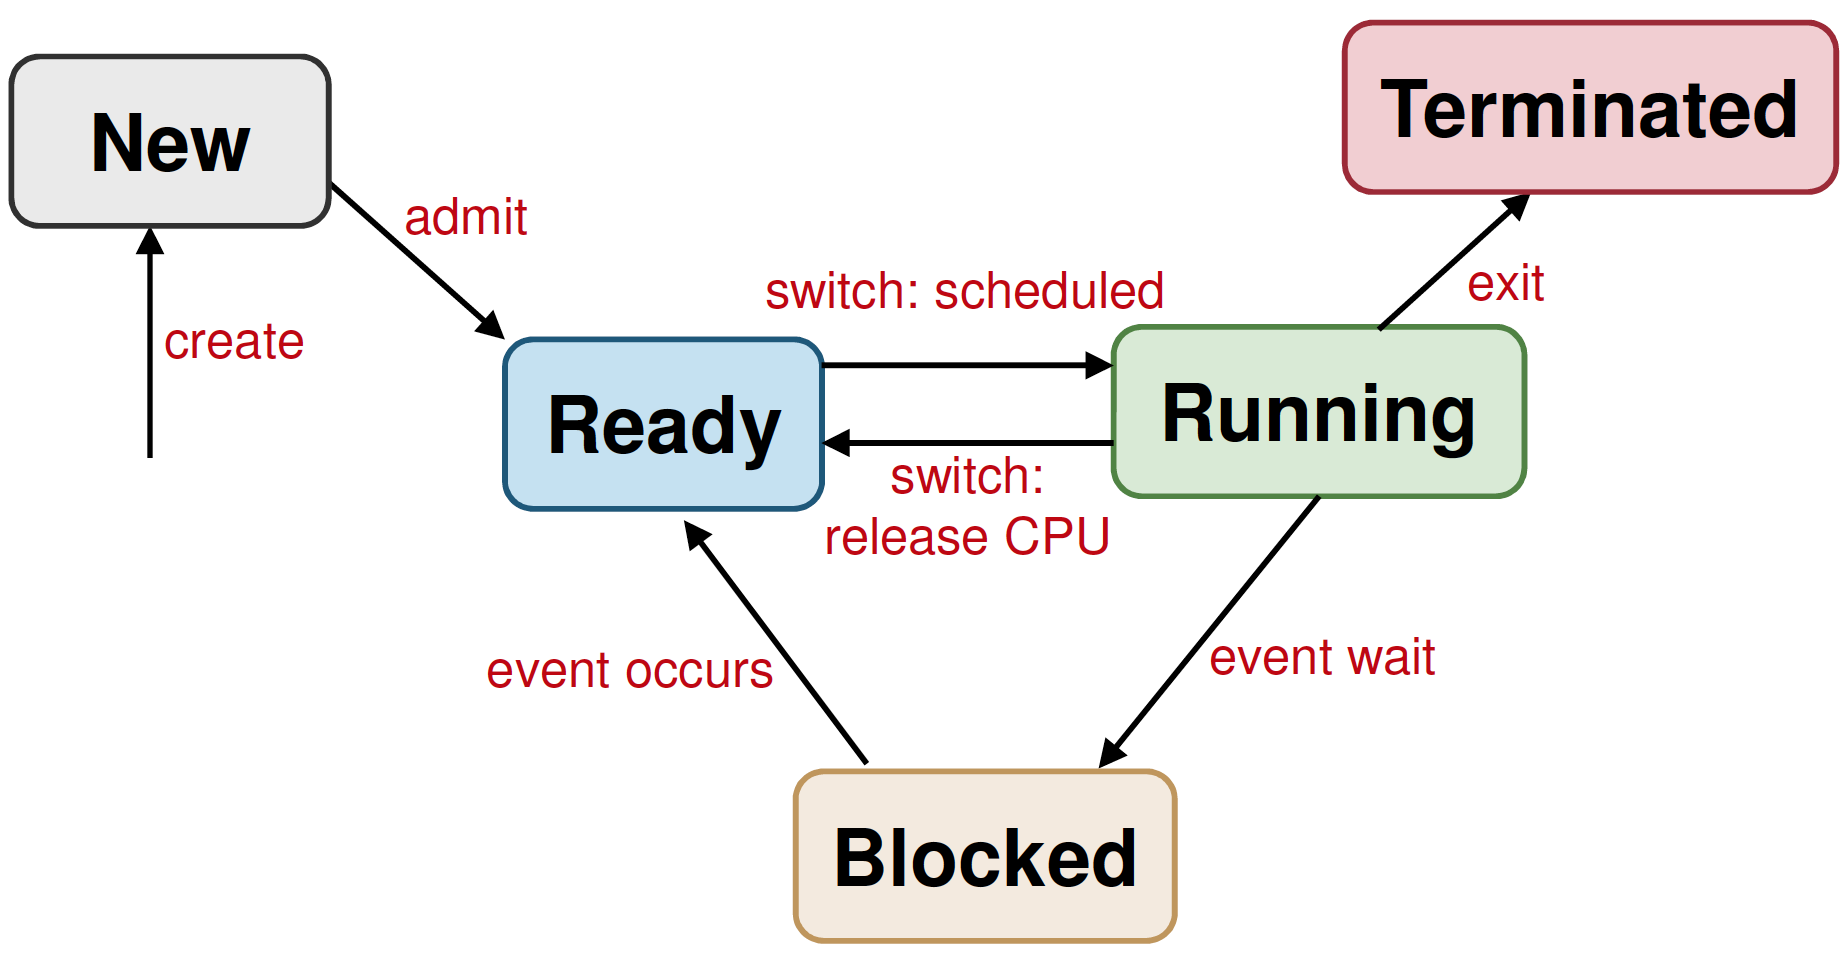
\includegraphics[width=\linewidth]{process-state}
  \end{tabularx}
  \begin{tabularx}{0.5\columnwidth}{X}
    \begin{itemize}
      \item 2 types of exec: time slicing (pseudo-parallelism), parallel execution of processes on different resources
      \item Create new process: \texttt{fork} or \texttt{exec(char *prog, char *argv)}
    \end{itemize}
  \end{tabularx}
  \textbf{Disadvantages}
  \begin{itemize}
    \item Creating a new process is costly (syscall overhead, all data structures must be allocated, initialised, copied)
    \item IPC is costly (must go through the OS)
  \end{itemize}
  \subsubsection{Threads}
  \begin{itemize}
    \item Share the address space of the process -- all threads belonging to the same process see the same value -> \textbf{shared-memory arch}
    \item Thread generation is faster than process generation
    \item Diff threads can be assigned to run on diff cores of a multicore
    \item 2 types:
          \begin{itemize}
            \item \textbf{User-level threads}: managed by a thread lib -- OS unaware of user-level threads. \textbf{Advantages:} switching thread context is fast, \textbf{Disadvantages:} OS cannot map diff threads of same process to diff exec resources -> no parallelism, OS cannot switch to another thread is 1 thread execs a blocking I/O op
            \item \textbf{Kernel threads}: OS is aware of existence.
            \item \textbf{Mapping User to Kernel Threads}
          \end{itemize}
    \item Global vars and all dynamically allocated data objects can be accessed by any thread
    \item Each thread has a private stack for function stack frames, existing iff the thread is active.
    \item No of threads should be suitable to parallelism degree of application, available execution resources, not too large to keep the overhead for thread creation, management, termination small
  \end{itemize}
  \subsection{Synchronisation}
  \begin{itemize}
    \item \textbf{Race condition} = 2 concurrent threads accessed a shared resource without any access synchronisation
    \item Use \textbf{mutual exclusion} to sync access to shared resources. Code sequence that uses mutex is called \textbf{critical section} (c.s.)
    \item Requirements:
          \begin{enumerate}
            \item \textbf{Mutual exclusion (mutex)}: if one thread is in the critical section, then no other is
            \item \textbf{Progress}: If some thread T is not in the critical section, then T cannot prevent some other thread S from entering the critical section. A thread in the critical section will eventually leave it
            \item \textbf{Bounded waiting (no starvation)}: If some thread T is waiting on the critical section, then T will eventually enter the critical section
            \item \textbf{Performance}: The overhead of entering \& exiting the critical section is small w.r.t. the work being done within it.
          \end{enumerate}
    \item \textbf{Starvation}: a process is prevented from making progressing because some other process has the resource it requires.
    \item \textbf{Deadlock} among a set of processes: if every process is waiting for an event that can be caused only by another process in the set. can arise when processes compete for access to limited resources, incorrectly synced.
    \item Condition for deadlock: if and only if these 4 conditions hold simultaneously:
          \begin{enumerate}
            \item \textbf{Mutex}: at least 1 resource must be held in non-sharable mode
            \item \textbf{Hold and wait}: There must be 1 process hilding 1 resource and waiting for another resource
            \item \textbf{No preemption} -- Resources cannot be preempted (critical sections cannot be aborted externally)
            \item \textbf{Circular wait} -- There must exist a set of processes $p_1, p_2, ... p_n$ such that $p_1$ is waiting for $p_2$, $p_2$ for $p_3$, so on.
          \end{enumerate}
    \item 4 Mechanisms:
  \end{itemize}
  \begin{enumerate}
    \item \textbf{Locks}
          \begin{itemize}
            \item 2 operations: \texttt{acquire()} to enter c.s., \texttt{release()} to leave c.s.
            \item Pair calls to acquire and release, can spin (\textbf{spinlock}) or block (\textbf{mutex})
          \end{itemize}
    \item \textbf{Semaphores}
          \begin{itemize}
            \item Abtract data type that provide mutex through atomic counters
            \item "Integers" that support 2 operations: \texttt{wait()} -- decrement, block until semaphore is open. \texttt{signal()}, increment, allow another thread to enter
            \item Safety property: semaphore value $\geq 0$
            \item 2 Types: Mutex/binary semaphore -- only 1 can enter c.s., Counting/general semaphore -- multiple can enter c.s.
            \item Drawback: shared global variable, no connection between the semaphore and the data being controlled, used for both c.s. (mutex) and coordination (scheduling), hard to use, prone to bugs
          \end{itemize}
    \item \textbf{Monitors}
          \begin{itemize}
            \item Guarantees mutex, only 1 thread can execute any monitor procedure at any time (the thread is "in the monitor")
            \item If 2nd thread invokes a monitor procedure when a 1st thread is alr executing, it blocks (monitor has to have a wait queue)
            \item If a thread within a monitor blocks, another one can enter
            \item Programming lang construct that controls access to shared data, added by compiler, enforced at runtime
            \item Encapsulates: Shared data structure, procedures that operate on the shared data structures, sync b/w concurrent threads that invoke the procedures
          \end{itemize}
    \item \textbf{Condition Variables}
          \begin{itemize}
            \item Support 3 operations: \texttt{wait()} -- release monitor lock, wait for condition var to be signalled, \texttt{signal()} wake up one waiting thread, \texttt{broadcast} wake up all waiting threads
          \end{itemize}
    \item \textbf{Barrier}
    \item \textbf{Messages}\\
          Simple model of communication \& sync based on atomic transfer of data across a channel, Direct application to distributed systems, Messages for synchronisation are straightforward
  \end{enumerate}
  \subsubsection{Classical Synchronisation Problems}
  Producer-consumer (finite, infinite buffer), Readers-writers, dining philosophers, barbershop
  \begin{enumerate}
    \item \textbf{Producer-consumer}
          \begin{verbatim}
    mutex = Semaphore(1)
    items = Semaphore(0)
    \end{verbatim}
          \begin{multicols*}{2}
            \begin{verbatim}
// Producer
event = waitForEvent()
// finite: spaces.wait()
mutex.wait()
buffer.add(event)
mutex.signal()
items.signal()
      \end{verbatim}
            \begin{verbatim}
// Consumer
items.wait()
mutex.wait()
event = buffer.get()
mutex.signal()
// finite: spaces.signal()
event.proces()
      \end{verbatim}
          \end{multicols*}
  \end{enumerate}
  \subsection{Implementing Locks}
  \begin{itemize}
    \item Implementation of locks has critical sections, therefore implementation of acquire/release must be atomic
    \item Need hardware support: atomic instruction (test-and-set), disable/enable interrupts (prevents context switches)
    \item \textbf{Test-and-set}: record old value, set value, return old value. Hardware executes atomically
  \end{itemize}
  \begin{minted}{C}
struct lock { int held = 0; }
void acquire(lock) { while(test_and_set(&lock->held)); }
void release(lock) { lock->held = 0; }
  \end{minted}
  \begin{itemize}
    \item \textbf{Problem}: spinlocks are wasteful -- a thread is spinning on a lock -> thread holding the lock cannot make progress on uniprocessor if lockholder yields/sleeps or involuntary context switch.
  \end{itemize}
  \section{Parallel Computing Platforms -- Arch Memory}
  \begin{itemize}
    \item Recap: $\text{CPU Time} = \frac{\text{Instructions}}{\text{Program}}\times\frac{\text{cycles}}{\text{instruction}}\times\frac{\text{seconds}}{\text{cycle}} = \frac{\text{seconds}}{\text{program}}$
    \item \textbf{Instruction/Program} affected by compiler \& ISA, \textbf{Cycles/Instruction} affected by processor implementation, \textbf{seconds/cycle} affected by clock speed (clock freq)
  \end{itemize}
  \subsection{Sources of processor performance gain: ($x$ parallelism, $x$ is ...)}
  \begin{itemize}
    \item \textbf{Bit level}: word size, larger so no need bitslicing
    \item \textbf{Instruction level}: \textbf{pipelining} (parallelism across time, split instruction execution in multiple stages, allow multiple instructions to occupy different stages in the same clock cycle given no data/control dependencies), \textbf{superscalar} (paralellism across space, duplicate pipelines, allow multiple instructions to pass through the same stage, dispatching multiple instructions to diff execution units in the processor, but scheduling is challenging (deciding which instructions can be executed together))
    \item \textbf{Thread level}: processor provides hardware support for the "thread context" -- information specific to each thread (PC, Registers, etc) so software threads can execute in parallel. E.g. SMT: Intel Hyper-threading
    \item \textbf{Process level} -- process has independent memory space, communicate with IPC through OS. can be mapped to multiple processor cores
    \item \textbf{Processor level}: \textbf{Shared memory}, \textbf{Distributed Memory}
  \end{itemize}
  \subsection{Flynn's Parallel Architecture Taxonomy}
  \textbf{SISD (Single Instruction Single Data)}: A single instruction stream is executed, each instruction work on single data. E.g. uniprocessor; \textbf{SIMD}
  A single instruction stream, working on multiple data, exploting data parallelism, known as vector processor. E.g. SSE, AVX in x86; \textbf{MISD}
  Multiple instruction streams, all instruction work on the same data at any time, no actual implementation; \textbf{MIMD} Each PU fetch its own instruction, each PU operates on its data. Most popular model for multiprocessor, \textbf{Variant -- SIMD + MIMD}
  Stream processor (GPU's): a set of threads executing the same code (SIMD), multiple set of threads executing in parallel (MIMD)
  \subsection{Memory Organisation}
  \begin{tabularx}{0.5\columnwidth}{X}
    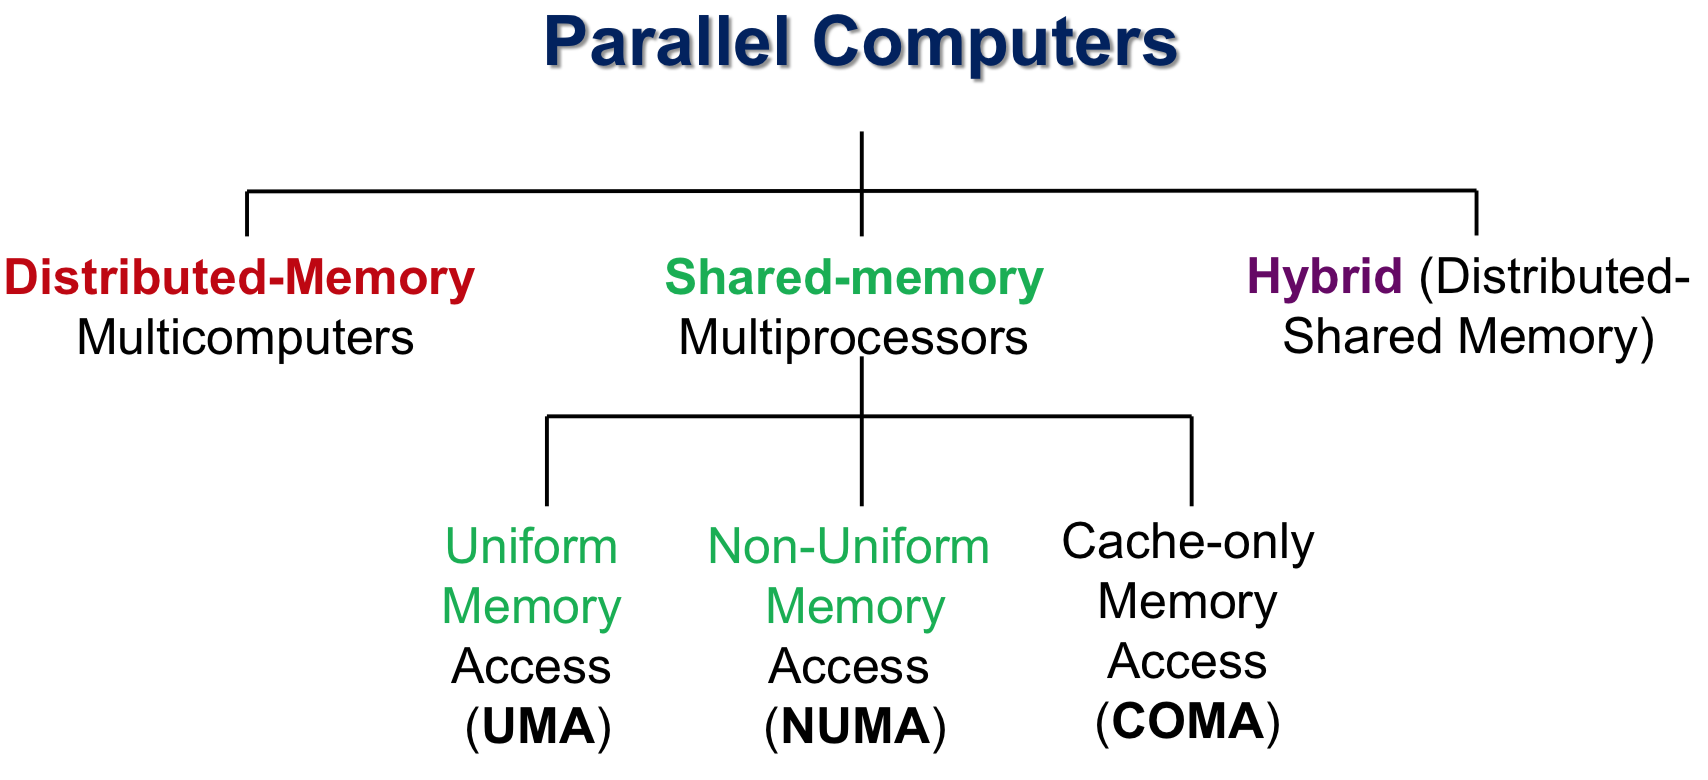
\includegraphics[width=\linewidth]{memory}
  \end{tabularx}
  \begin{tabularx}{0.5\columnwidth}{X}
    \subsubsection{CC (Cache Coherence Protocol)}
    e.g. ccNUMA, each node has cache memory to reduce contention
  \end{tabularx}
  \subsubsection{COMA (Cache Only Memory Architecture)}
  Each memory block works as cache memory, data migrates dynamically and continuously according to the cache coherence scheme
  \subsubsection{UMA (Uniform Memory Access)}
  Latency of accessing the main memory is uniform for every processor, suitable for small number of processors
  \subsubsection{NUMA (Non-Uniform Memory Access)}
  Diagram just like Distributed-Memory system
  \begin{itemize}
    \item Physically distributed memory of all processing elements are combined to form a global shared-memory address space, also called distributed shared-memory.
    \item Accessing local mem faster than remote mem for a processor.
  \end{itemize}
  \subsubsection{Distributed-Memory System}
  \begin{tabularx}{0.5\columnwidth}{X}
    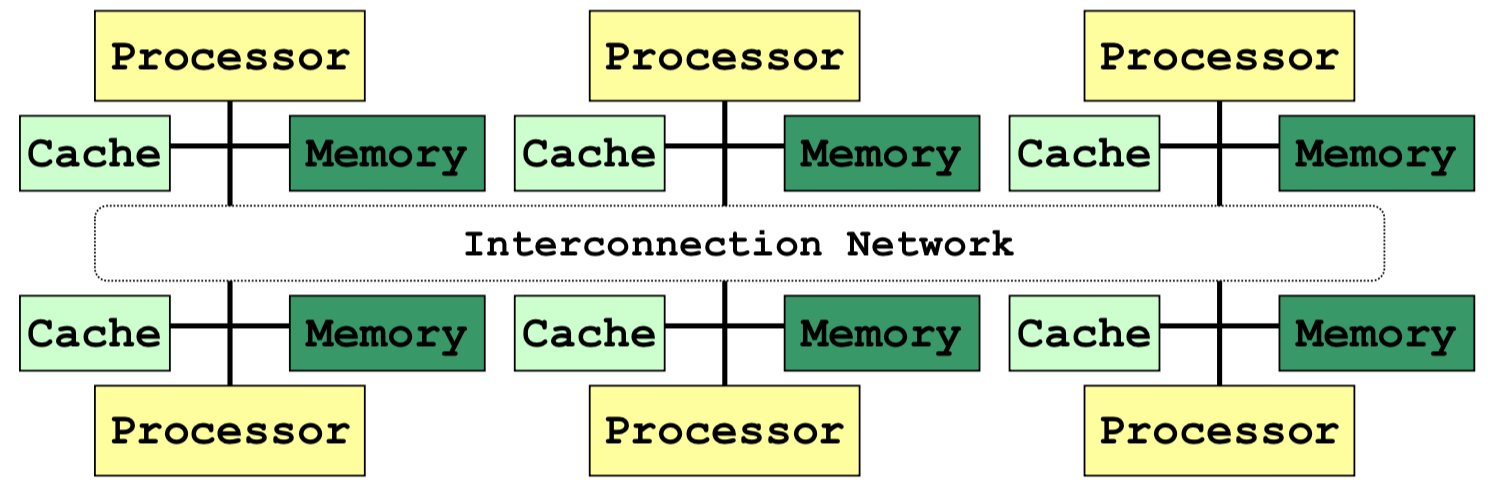
\includegraphics[width=\linewidth]{distributed}
  \end{tabularx}
  \begin{tabularx}{0.5\columnwidth}{X}
    Each node is an independent unit with processor, memory and peripheral elements.
  \end{tabularx}
  \begin{itemize}
    \item Physically distributed memory module: mem in a node is private
    \item Data exchanges between nodes with message-passing
  \end{itemize}
  \subsubsection{Shared Memory System}
  \begin{tabularx}{0.5\columnwidth}{X}
    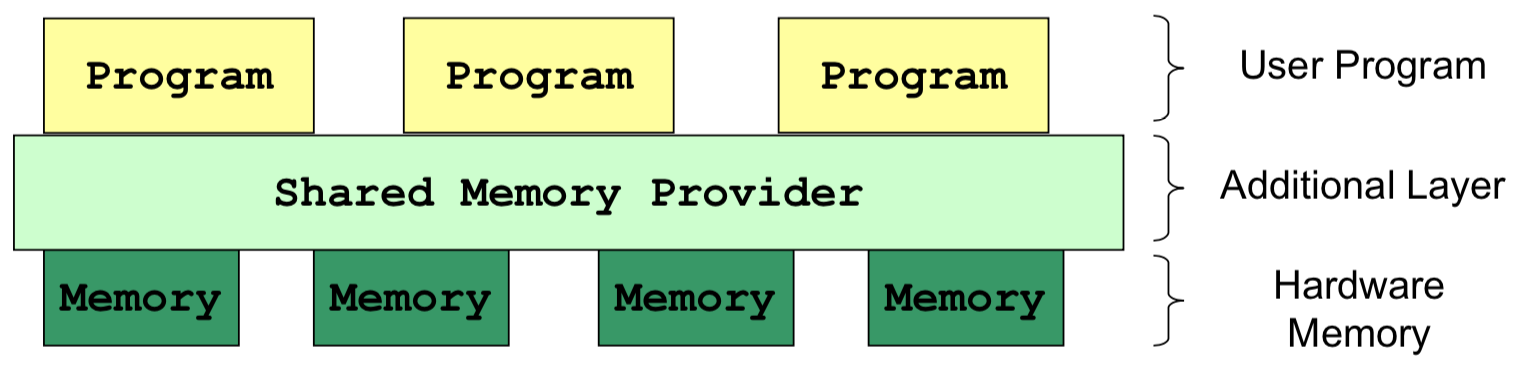
\includegraphics[width=\linewidth]{shared}
  \end{tabularx}
  \begin{tabularx}{0.5\columnwidth}{X}
    Access memory through shared memory provider which maintain the illusion of shared memory.
  \end{tabularx}
  \begin{itemize}
    \item Program is unaware of the actual hardware memory architecture
    \item Data exchange between nodes with shared variables
    \item \textbf{Advantages}: no need to partition code/data or physically move data among processors -> communication is efficient
    \item \textbf{Disadvantages}: Special synchronisation constructs are required, lack of scalability due to contention
  \end{itemize}
  \subsubsection{Hybrid (Distributed-Shared Memory)}
  \begin{tabularx}{0.8\columnwidth}{X}
    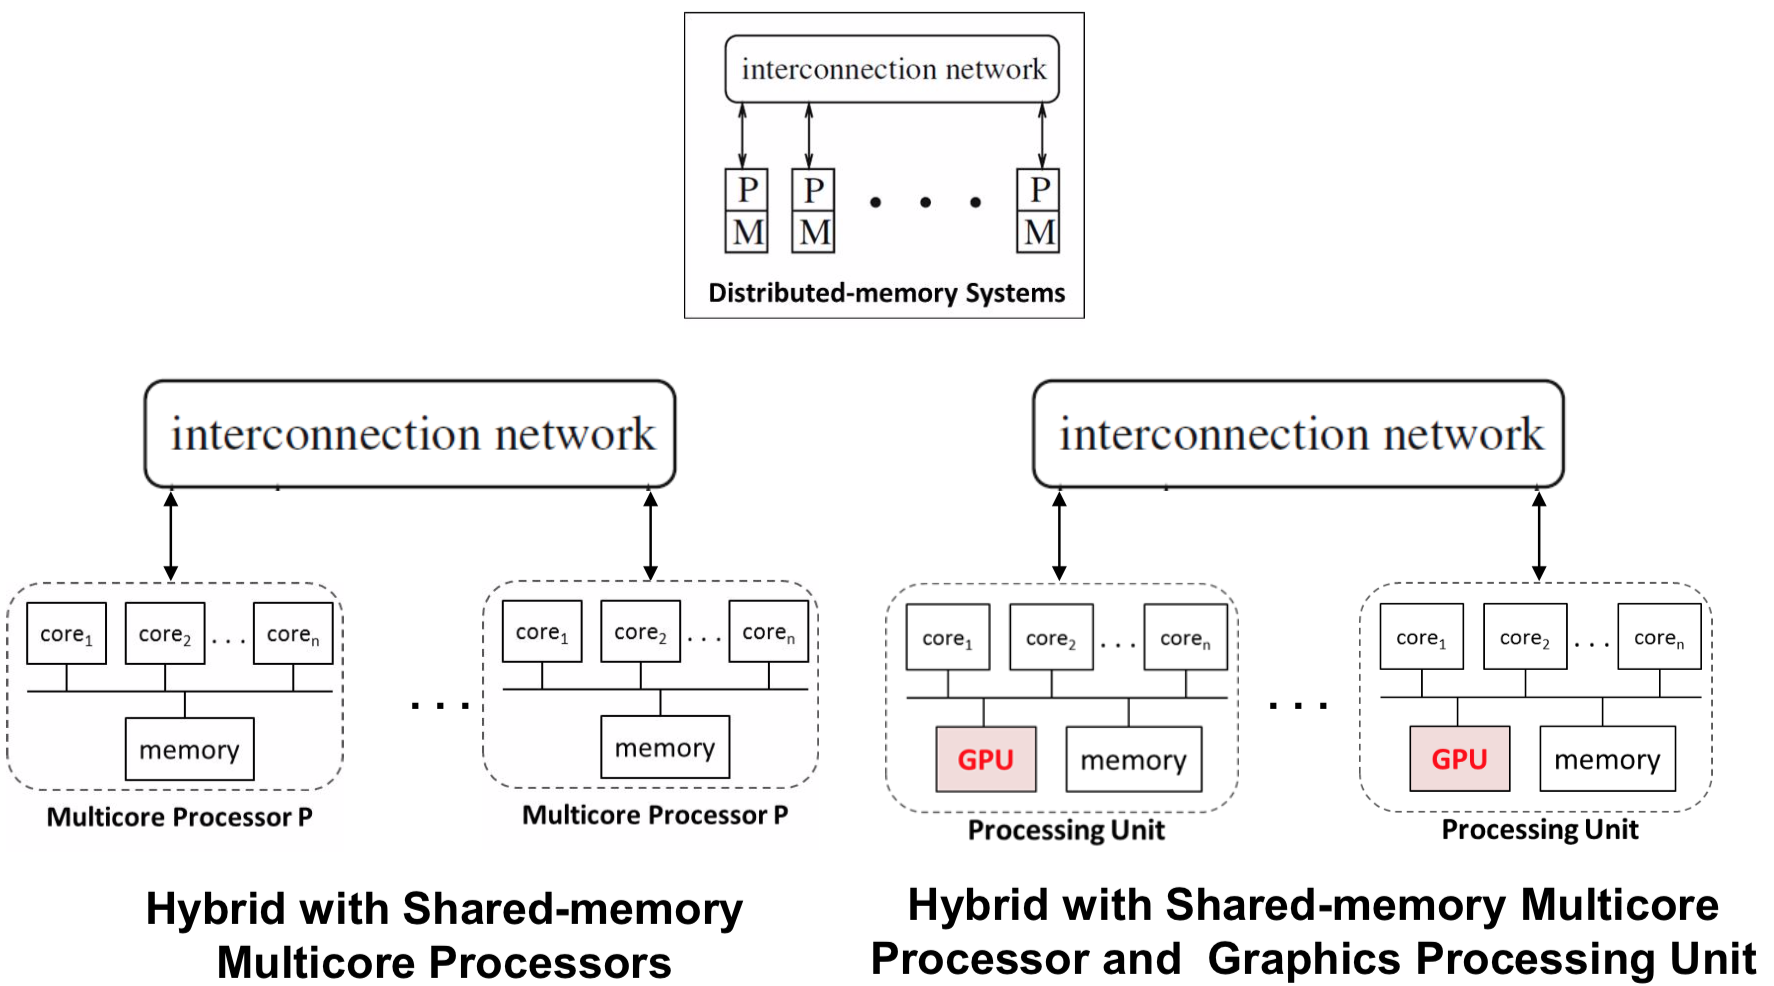
\includegraphics[width=\linewidth]{distributed-shared}
  \end{tabularx}
  \begin{tabularx}{0.17\columnwidth}{X}
    e.g. Hybrid with GPU
  \end{tabularx}
  \subsection{Multicore Architecture}
  \subsubsection{Hierarchical Design}
  \begin{itemize}
    \item Multiple cores share multiple caches, cache size increases from the leaves to the root.
    \item Usages: standard desktop, server processors, GPUs
  \end{itemize}
  \subsubsection{Pipelined Design}
  \begin{itemize}
    \item Data elements are processed by multiple execution cores in a \textbf{pipelined} way, from one core to the next
    \item Useful if same computation steps have to be applied to a long sequence of data elements, e.g. network processors used in routers and graphic processors
  \end{itemize}
  \subsubsection{Network-based Design}
  \begin{itemize}
    \item Cores and their local caches and memories are connected via an interconnection network
  \end{itemize}
  \section{Parallel Programming Models}
  Common classification:
  \begin{itemize}
    \item \textbf{Level of parallelism}: granulaty from instruction -> statement -> procedural (function/methods) level or parallel loops
    \item \textbf{Specification of parallelism}: implicit/user-defined explicit
    \item \textbf{Execution}: e.g. SIMD/SPMD, sync or async
    \item \textbf{Communication mode}: message-passing/shared vars
    \item \textbf{Synchronisation (coordination mechanisms)}
  \end{itemize}
  \subsection{Decomposition}
  \begin{itemize}
    \item Generate enough tasks to keep all cores busy at all times (no of tasks $\geq$ no of cores)
    \item Granularity is large compared to scheduling \& mapping time (size of task $>>$ overhead of parallelism)
    \item \textbf{Static} at program start/compile time, \textbf{Dynamic} during runtime
  \end{itemize}
  \subsection{Scheduling}
  \begin{itemize}
    \item Find an efficient task exec order to optimise a given objective.
    \item Good load balancing among tasks: Computations, Memory accesses (shared), Communication ops (distributed)
    \item Static/Dynamic scheduling
  \end{itemize}
  \subsection{Mapping}
  \begin{itemize}
    \item Assignment of processes/threads to execution units
    \item Focuses on performance: Equal utilisation of execution units, minimal communication between the processors
  \end{itemize}
  \subsection{Parallelism}
  \begin{itemize}
    \item Avg no of units of work that can be performed in parallel/unit time. Work = task + dependencies.
    \item Types in increasing task size: instruction -> loop -> data -> task
  \end{itemize}
  \subsubsection{Instruction Parallelism}
  Multiple instructions exec may be inhibited by 3 types of data deps. Can be used to create data dependency graph
  \begin{itemize}
    \item \textbf{Flow dep (RAW)}/ true dependency: (\textbf{a}) \texttt{a = b + c; e = a + d}
    \item \textbf{Anti-dependency (WAR)}: (\textbf{b}) \texttt{a = b + c; b = d + e;}
    \item \textbf{Output dep (WAW)}: (\textbf{a}) \texttt{a = b + c; a = d + e;}
  \end{itemize}
  \subsubsection{Loop Parallelism}
  If the iterations are independent, they can be executed in arbitrary order \& in parallel on different processors
  \subsubsection{Data Parallelism}
  \begin{itemize}
    \item \textbf{Partition the data} used in solving the problem among the processing units; each processing unit carries out similar operations on its part of the data
    \item Same op is applied to diff elements of a data set, if ops are independent, elements can be distributed among processors for parallel execution, or using SIMD computers/instructions
    \item e.g. \texttt{for (i = 0; i < N; i++) a[i] = b[i - 1] + c[i];}
    \item On MIMD, common model: SPMD (Single Program Multiple Data) -- 1 parallel program is executed by all processors in parallel (both shared \& distributed address space)
  \end{itemize}
  \subsubsection{Task Parallelism}
  \begin{itemize}
    \item \textbf{Partition tasks} in solving the problem among processing units
  \end{itemize}
  \subsection{Task Dependence Graph}
  \begin{itemize}
    \item A directed acyclic graph, \textbf{node}: task, value = expected exec time; \textbf{edge}: control dep b/w task
    \item \textbf{Properties}:
          \begin{itemize}
            \item \textbf{Critical Path Length}: min (fastest) completion time
            \item \textbf{Degree of concurrency} = total work / critical path length (indication of amount of work that can be done concurrently)
          \end{itemize}
  \end{itemize}
  \subsection{Representation of parallelism}
  %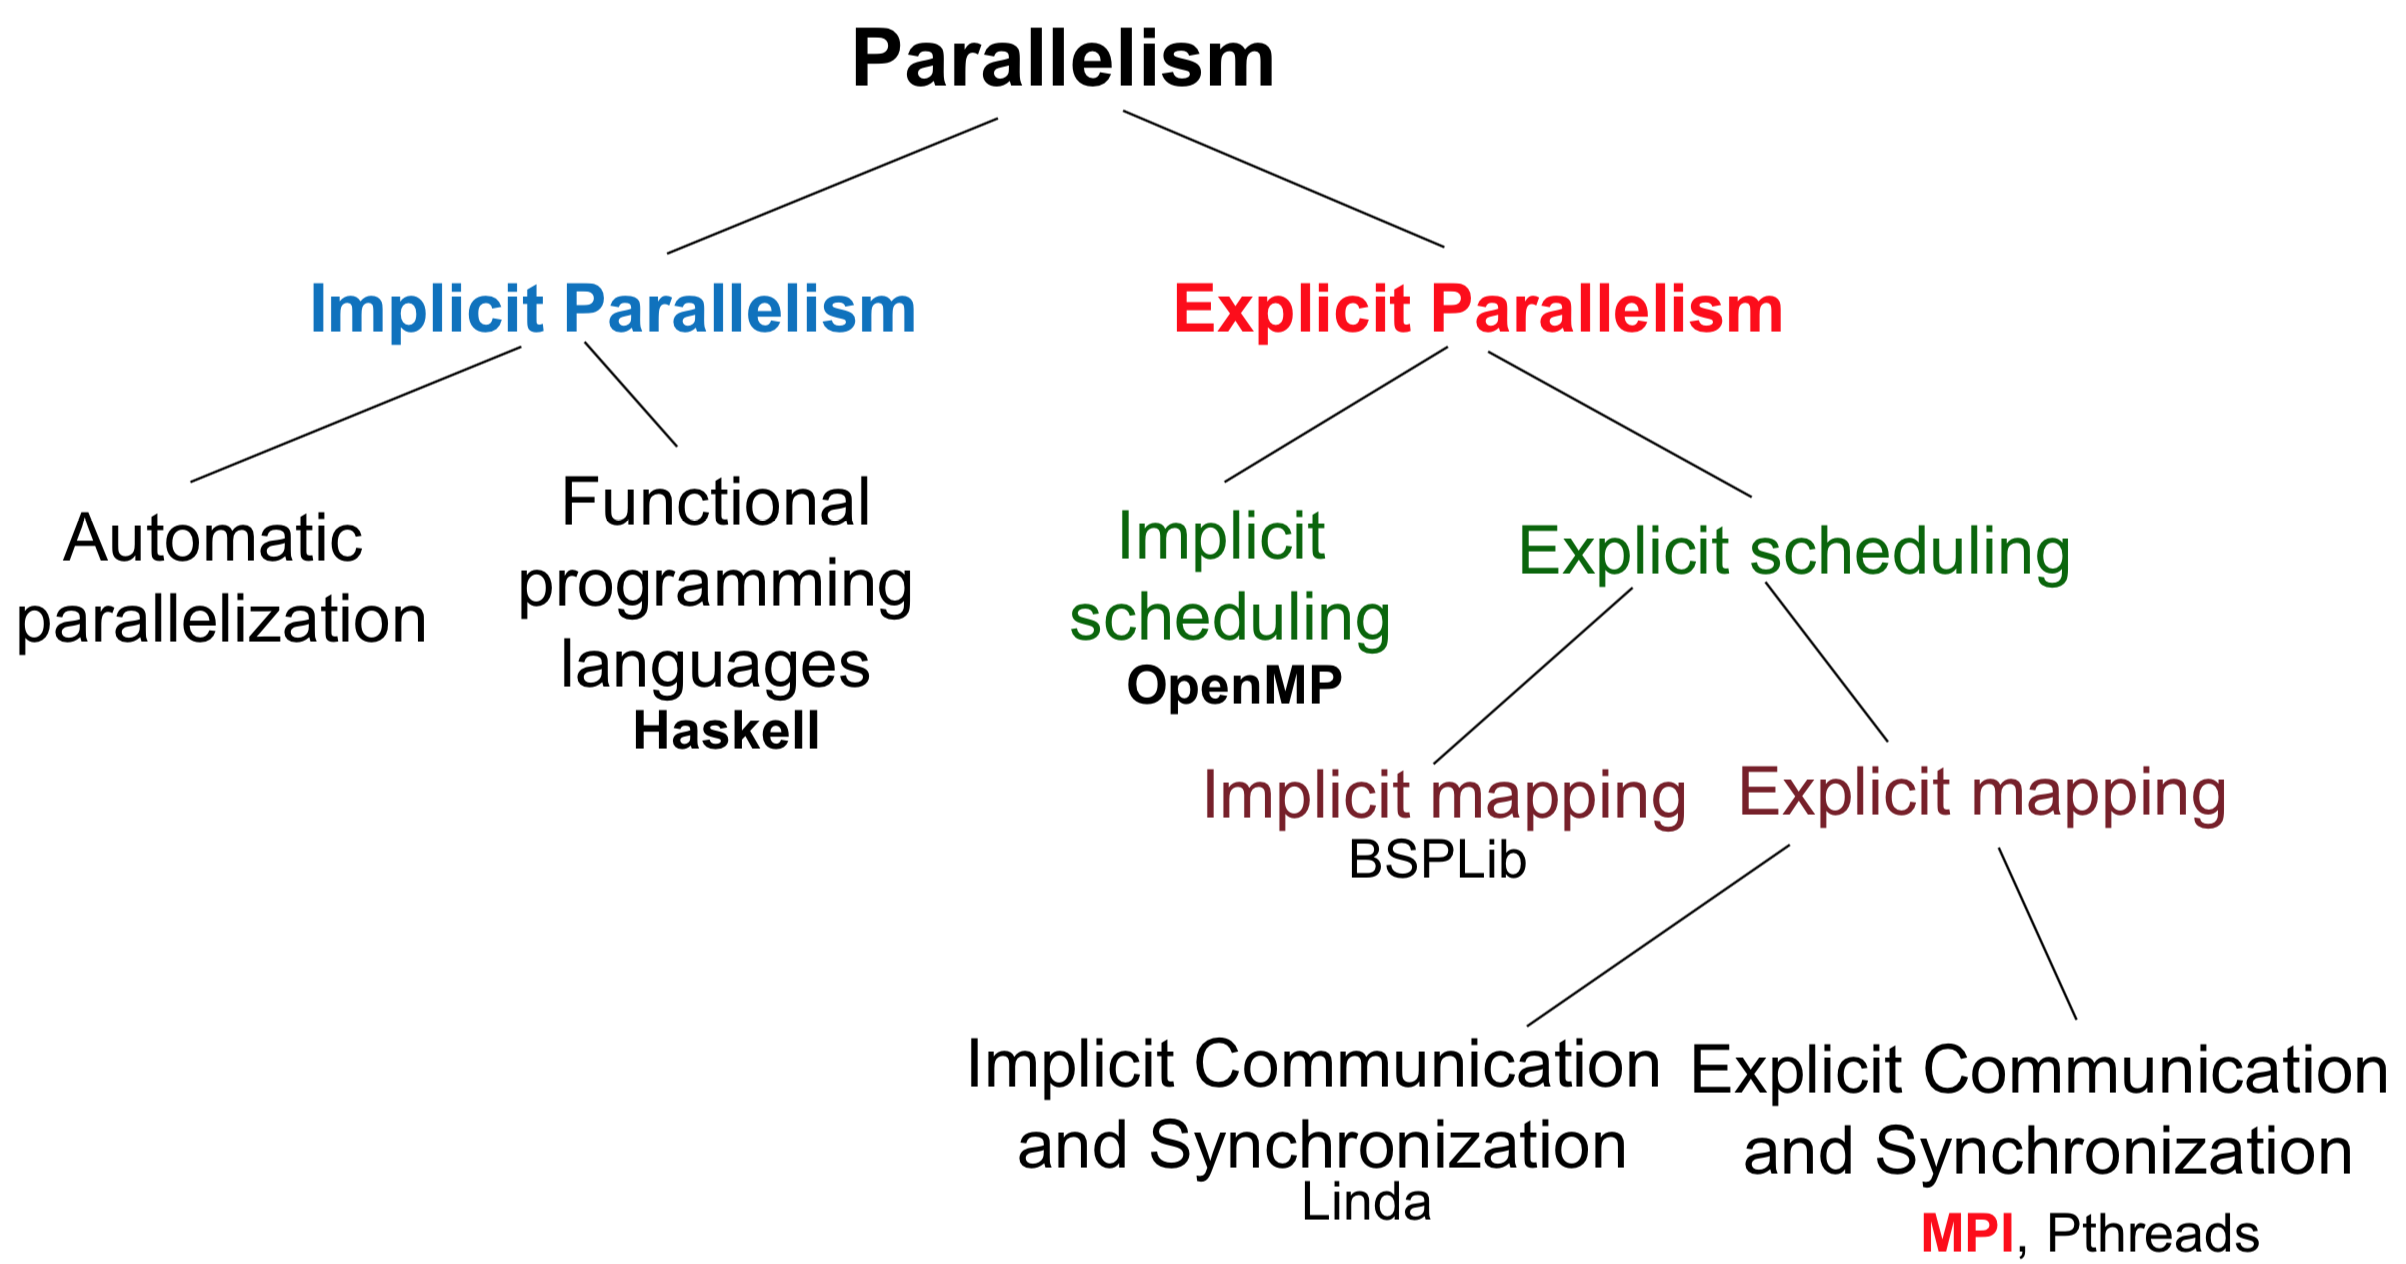
\includegraphics[width=0.55\linewidth]{parallelism-rep}
  \subsubsection{Automatic Parallelisation}
  \begin{itemize}
    \item Parallelising compilers perform decomposition \& scheduling
    \item Drawbacks: Dep analysis is difficult for pointer-based computations/indirect addressing; Exec time of function calls/loops with unknown bounds is difficult to predict at compile time
  \end{itemize}
  \subsubsection{FP languages}
  \begin{itemize}
    \item Describe computation as eval of maths functions w/o side effects.
    \item \textbf{Advantage}: new lang constructs are not necessary to enable parallel exec, \textbf{Challenge}: extract parallelism at right level of recursion
  \end{itemize}
  \subsection{Parallel Programming Patterns}
  Provides a coordination structure for tasks
  \subsubsection{Fork-Join}Task T creates a number of child tasks with \texttt{fork()}, then waits for termination using \texttt{join} call
  \subsubsection{Parbegin-Parend}
  When an executing thread reaches parbegin-parend, a set of threads is created and statements of the construct are assigned to these threads for execution. Statements following the construct are only executed after all these threads have finished their work.
  \subsubsection{SIMD}
  Single instructions are executed synchronously by the different threads on different data
  \subsubsection{SPMD}
  Same program executed on different processors but operate on different data, No implicit synchronisation -- must use explicit sync ops
  \subsubsection{Master-Slave (or Master-Worker)}
  Master coord, init, timings, output, assigns work to slaves
  \subsubsection{Client-Server}
  \begin{itemize}
    \item MPMD (multiple program multiple data) model
    \item Useful in heterogeneous systems
    \item Server compute requests from multiple client tasks concurrently, can use multiple threads to compute a single request
    \item A task can generate request to other tasks (client role) and process requests from other tasks (server role)
  \end{itemize}
  \subsubsection{Pipelining}
  Data in the application is partitioned into a stream of data elements that flows through the each of the pipeline tasks one after the other to perform different processing steps.
  \subsubsection{Task (Work) Pools}
  \begin{itemize}
    \item Common data structure from which threads can access to retrieve tasks for execution. During processing of a task, a thread can generate new tasks and insert them into the task pool.
    \item No of threads is fixed, threads created statically by main thread
    \item Access to the task pool must be synced to avoid race conditions
    \item Exec is completed when Task pool is empty, Each thread has terminated the processing of its last task
    \item \textbf{Advantages}: Useful for adaptive \& irregular applications (tasks can be generated dynamically), Overhead for thread creation is independent of problem size \& no of tasks
    \item \textbf{Disadvantages}: For fine-grained tasks, the overhead of retrieval \& insertion of tasks becomes important
  \end{itemize}
  \subsubsection{Producer-Consumer}
  \begin{itemize}
    \item Prod threads produce data which are used as input by con threads
    \item Sync must be used to ensure correct coordination b/w prod \& con
  \end{itemize}
  \section{Performance of Parallel Systems}
  \subsection{Performance factors}
  Down the list, Higher level of abstraction, higher loss in performance
  \begin{itemize}
    \item \textbf{Machine Model}: provide a description of hardware \& OS
    \item \textbf{Architectural Model}: includes interconnection network, memory org, sync/async processing, exec mode
    \item \textbf{Computational Model}: provide an analytical method for designing and evaluating algo on a given arch model
    \item \textbf{Programming Model}: define how programmer can code an algo
  \end{itemize}
  \subsubsection{Reponse Time in Sequential Systems}
  \begin{itemize}
    \item Wall-clock time (actual time taken) = user CPU + system CPU (exec OS routines) + waiting time (I/O, time sharing)
    \item Focus on CPU Time: depends on Translation of program statements by compiler, exec time of each instruction
    \item $Time_{user}(A) = N_{cycle}(A) \times Time_{cycle}$, $N_{cycle}(A) = \sum\limits_{i = 1}^{n} n_i(A)\times CPI_i$
    \item Thus, $Time_{user}(A) = N_{instr}(A)\times CPI(A) \times Time_{cycle}$
    \item Refinement with memory access time:\\
          $Time_{user}(A) = (N_{cycle}(A) + N_{mm\_cycle}(A)) \times Time_{cycle}$
    \item One-level cache: $N_{mm\_cycle}(A) = N_{read\_cycle}(A) + N_{write\_cycle}(A)$, $N_{read\_cycle}(A) = N_{read\_op}(A)\times R_{read\_miss}(A) \times N_{miss\_cycles}(A)$
    \item $Time_{user}(A) = (N_{instr}(A)\times CPI(A)) + N_{rw\_op}(A)\times R_{miss}(A) \times N_{miss\_cycles} \times Time_{cycle}$ ($R_{miss}(A)$ r/w miss rate)
    \item \textbf{Average memory access time}:\\
          $T_{read\_access}(A) = T_{read\_hit} + R_{read\_miss}(A) \times T_{read\_miss}$
    \item \textbf{Two-level cache}:\\
          $T_{read\_access}(A) = T^{L1}_{read\_hit} + R^{L1}_{read\_miss}(A) \times T^{L1}_{read\_miss}$\\
          $T^{L1}_{read\_miss}(A)= T^{L2}_{read\_hit}(A) + R^{L2}_{read\_miss}(A) \times T^{L2}_{read\_miss}$\\
          Global miss rate = $R^{L1}_{read\_miss}(A) \times R^{L2}_{read\_miss}(A)$
  \end{itemize}
  \subsubsection{Throughput: MIPS (Million-Instruction-Per-Second)}
  \begin{itemize}
    \item $MIPS(A) = \frac{N_{instr}(A)}{Time_{user}(A)\times 10^6} = \frac{clock freq}{CPI(A) \times 10^6}$
    \item \textbf{Drawbacks}: Consider only the no of instr, easily manipulated
  \end{itemize}
  \subsubsection{Million-FLoating-point-Operations-Per-Second}
  \begin{itemize}
    \item $MFLOPS(A) = \frac{N_{flops}(A)}{Time_{user}(A) \times 10^6}$
    \item \textbf{Drawbacks}: No differentiation between diff types of flops
  \end{itemize}
  \subsubsection{Benchmarks}
  \textbf{Industry Standards}: SPEC benchmark suites, EEMBC benchmark suites, Numerical Aerodynamic Simulation (NAS) from NASA (massively parallel benchmark for computer cluster), \textbf{Simple Benchmark}: Linpack, Dhrystone/Whetstone, Tak function
  \subsection{Parallel Execution Time}
  \begin{itemize}
    \item $T_p(n)$, problem of size $n$, $p$ processors
    \item Consists of Time for executing local computations, exchange of data and sync b/w processors, waiting time (unequal load distribution, wait to access shared data structure)
  \end{itemize}
  \subsubsection{Cost}
  \begin{itemize}
    \item $C_p(n) = p \times T_p(n)$ = total amount of work performed by all processors (processor-runtime product)
    \item \textbf{Cost optimal} = execs same total no of ops as fastest seq program
  \end{itemize}
  \subsubsection{Speedup}
  \begin{itemize}
    \item $S_p(n) = \frac{T_{best\_seq}(n)}{T_p(n)}$
    \item Theoretically, $S_p(n) \leq p$ always holds, but in practice $S_p(n)>p$ (superlinear speedup) can occur (due to better cache locality, etc.)
  \end{itemize}
  \subsubsection{Best Sequential Algo: Difficulties}
  \begin{itemize}
    \item Best sequential algo may not be known OR there exists an algo with optimum asymptotic exec time, but other algo lead to lower exec time in practice
  \end{itemize}
  \subsection{Parallel Program Efficiency}
  $E_p(n) = \frac{T_{best\_seq}}{C_p(n)} = \frac{S_p(n)}{p} = \frac{T_{best\_seq}}{p\times T_p(n)}$, Ideal $S_p(n) = p \rightarrow E_p(n) = 1$
  \subsection{Scalability}
  \subsubsection{Grosch's Law (1953)}
  The speed of a computer is proportional to the square of its cost
  \begin{itemize}
    \item A collection of smaller processors will always have less performance than a single processor of the same total cost
    \item Rebuttal: No longer applies to computer systems build with many inexpensive commodity processors, Commodity processors are more cost effective than custom design supercomputers
  \end{itemize}
  \subsubsection{Minsky's Conjecture (1971)}
  The speedup achievable by a parallel computer increases as the logarithm of the no of processing elements
  \begin{itemize}
    \item Implication: large-scale parallelism unproductive
    \item Rebuttal: Experimental results prove that speedup depends strongly on particular algo \& computer arch, and many algo exhibit linear speedup for over 100 processors
  \end{itemize}
  \subsubsection{Amdahl's Law (1967)}
  Speedup of parallel execution is limited by the fraction of the algorithm that cannot be parallelised
  \begin{itemize}
    \item $0 \leq f \leq 1$ = sequential fraction (fixed-workload performance)
    \item $S_p(n) = \frac{T_{best\_seq}(n)}{f\times T_{best\_seq}(n)+\frac{1-f}{p}T_{best\_seq}(n)}$
    \item Implication: manufacturers are discouraged from making large parallel computers, more research attn shifted towards developing parallelising compilers that reduces $f$
    \item Rebuttal: in many computing problems, $f$ is not constant, dependent on problem size $n$. An effective parallel algorithm is $\lim\limits_{n\rightarrow\infty}f(n) = 0$, thus speedup $\lim\limits_{n\rightarrow\infty}S_p(n)=\frac{p}{1+(p-1)f(n)}=p$, thus Amdahl's law can be circumvented for large problem size
  \end{itemize}
  \subsubsection{Gustafson's Law (1988)}
  \begin{itemize}
    \item Main constraint is exec time, then higher computing power is used to improve accuracy/better result
    \item If $f$ decreases when $n$ increases, then $S_p(n) \leq p$, $\lim\limits_{n\rightarrow\infty}S_p(n)=p$
  \end{itemize}
  \section{Coherence, Consistency, Interconnections}
  \subsection{Cache}
  \subsubsection{Write Policy}
  \begin{itemize}
    \item \textbf{Write-through} - write immediately transferred to main memory, Advantage: no stale value, disadv: slow (soln: use a write buffer)
    \item \textbf{Write-back} - write op performed only in the cache, write performed only when cache block is replaced, tracked with a dirty bit. Adv: less write ops, disadv: mem may contain invalid entries
  \end{itemize}
  \subsubsection{Cache Coherence Problem}
  3 properties of coherent memory system:
  \begin{enumerate}
    \item $P$ write to $X$, no write to $X$, $P$ read from $X$, should be same value
    \item $P_1$ write to $X$, no write ro $X$, $P_2$ read from $X$, should be same value (\textbf{Write Propagation})
    \item Write $v_1$ to $X$, write $v_2$ to $X$, processors read in same order ($v_1$ then $v_2$) (\textbf{Write Serialisation})
  \end{enumerate}
  \subsubsection{Maintaining cache coherence}
  \begin{itemize}
    \item Software-based soln (compiler+hw aided soln)
    \item Hardware-based soln (most common on multiprocessor, known as \textbf{cache coherence protocols})
  \end{itemize}
  Major Tasks:
  \begin{itemize}
    \item \textbf{Track cache line sharing status}, 2 major categories:
          \begin{itemize}
            \item \textbf{Snooping-based}: no centralised directory, each cache keeps track of the sharing status, cache \textbf{monitors/snoops} on the bus to update the status of cache line \& take appropriate action. Most common in arch with a bus. Granularity is cache block.
                  \begin{itemize}
                    \item All the processors on the bus can observe every bus transactions (\textbf{write propagation}), Bus transactions visible to the processors in the same order (\textbf{write serialisation})
                  \end{itemize}
            \item \textbf{Directory based}: sharing status kept in a centralised location. Most common in NUMA
          \end{itemize}
    \item Handle the update to a shared cache line (maintain coherence)
  \end{itemize}
  \subsection{Memory Consistency Models}
  4 types of memory op orderings: RAW, RAR, WAR, WAW
  \subsubsection{Sequential Consistency}
  Maintains all four orderings
  \begin{itemize}
    \item Every processor issues its mem ops in program order
    \item Mem accesses are atomic (effect of each mem op must be visible to all before next mem op)
  \end{itemize}
  \subsubsection{Total Store Ordering (TSO)}
  \begin{itemize}
    \item Relaxing RAW (WAW still exists, writes by same thread in-order)
    \item Processor $P$ can read $B$ before its write to $A$ is seen by all (processor can move its own reads in front of its own writes)
    \item Read by other processors cannot return new value of $A$ until write to $A$ is observed by all processors
  \end{itemize}
  \subsubsection{Processor Consistency}
  \begin{itemize}
    \item Relaxing RAW (WAW still exists, writes by same thread in-order)
    \item Any processor can read new value of $A$ before the write is observed by all processors
  \end{itemize}
  \subsubsection{Partial Store Ordering}
  \begin{itemize}
    \item Relaxing RAW \& WAW, but still guarantees write atomicity
  \end{itemize}
  \subsection{Interconnection Networks}
  \subsubsection{Shearsort}
  \begin{enumerate}
    \item Row sorting, odd rows sort asc, even rows sort desc
    \item Column sorting, all columns sort asc
    \item Repeat until sorted
  \end{enumerate}
  For $n$ numbers, $log(n)$ phases, $O(\sqrt{n}\log n)$. Good for 2D mesh network, only communication with adjacent nodes.
  \subsection{Topology}
  \subsubsection{Metric}
  \begin{itemize}
    \item \textbf{Diameter}: max. distance b/w any pair of nodes (small diameter, small distances for message transmission)
    \item \textbf{Degree}: no of direct neighbour nodes (small node degree reduces node h/w overhead)
    \item \textbf{Bisection width}: min. no. of edges to be removed to divide the network into 2 equal halves. (measure for capacity of network when transmitting messages simulatenously)
    \item \textbf{Node connectivity}: min. no of nodes failing to disconnect the network (robustness of the network)
    \item \textbf{Edge connectivity}: min. no of edges failing to disconnect the network (no of independent paths b/w any pair of nodes)
  \end{itemize}
  \subsubsection{Direct Interconnection (Static/Point-To-Point)}
  Torus = 2 links for every dim, Mesh = torus w/ no wraparound, CCC = k-dim hypercube but each node replaced with cycle of k-nodes\\
  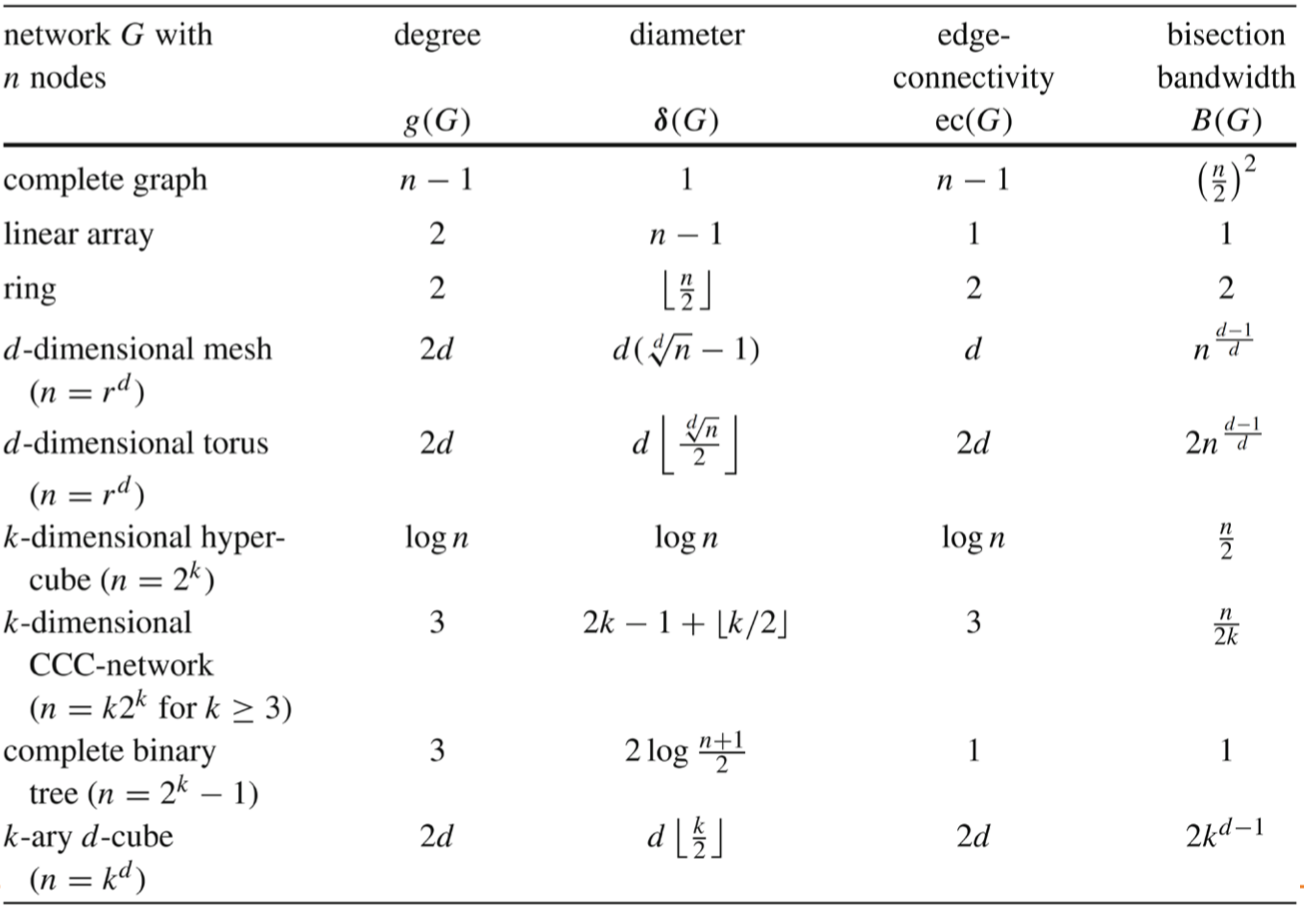
\includegraphics[width=\linewidth]{topology}
  \subsubsection{Indirect Interconnection (using switches)}
  \begin{itemize}
    \item \textbf{Bus Network} -- a set of wires, only one pair of devices can communicate at a time, bus arbiter for coordination
    \item \textbf{Crossbar Network} has $n\times m$ switches for $n$ inputs, $m$ outputs. Switch either straight/change dir
    \item \textbf{Omega Network} -- 1 unique path for every input to output, Uses $\log n$ stages, $\frac{n}{2}$ switches/stage. Edge from node $(\alpha, i)$ to two nodes $(\beta, i + 1)$ where $\beta = \alpha$ by a cyclic left shit (+ inversion of the LSBit)
    \item \textbf{Butterfly Network} -- Node $(\alpha, i)$ connects to $(\alpha, i + 1)$ and $(\alpha', i + 1)$, $\alpha$ and $\alpha'$ differ in the (i+1)th bit from the left (cross edge)
    \item \textbf{Baseline Network} -- Node $(\alpha, i)$ connects to 2 nodes $(\beta, i + 1)$ where $\beta = $ cyclic right shift of last (k-1) bits of $\alpha$ OR inversion of the LSBit of $\alpha$ + cyclic right shift of last (k-i) bits.
  \end{itemize}
  \begin{tabularx}{0.32\linewidth}{X}
    Omega \\
    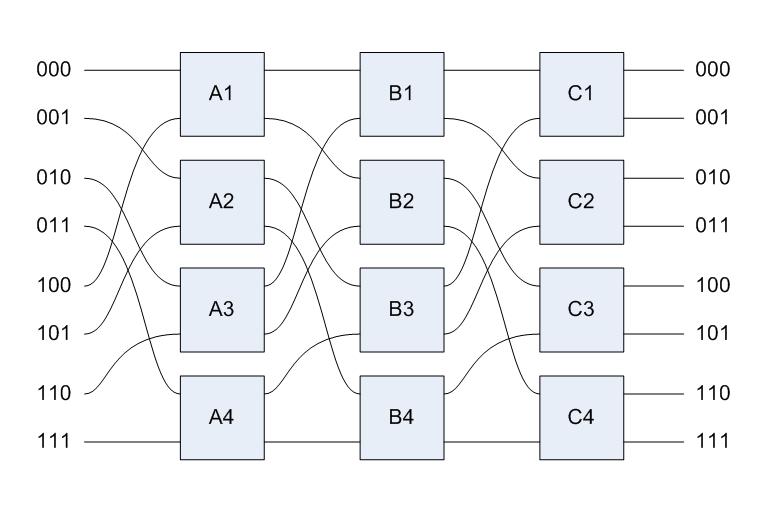
\includegraphics[width=\linewidth]{omega}
  \end{tabularx}
  \begin{tabularx}{0.32\linewidth}{X}
    Butterfly \\
    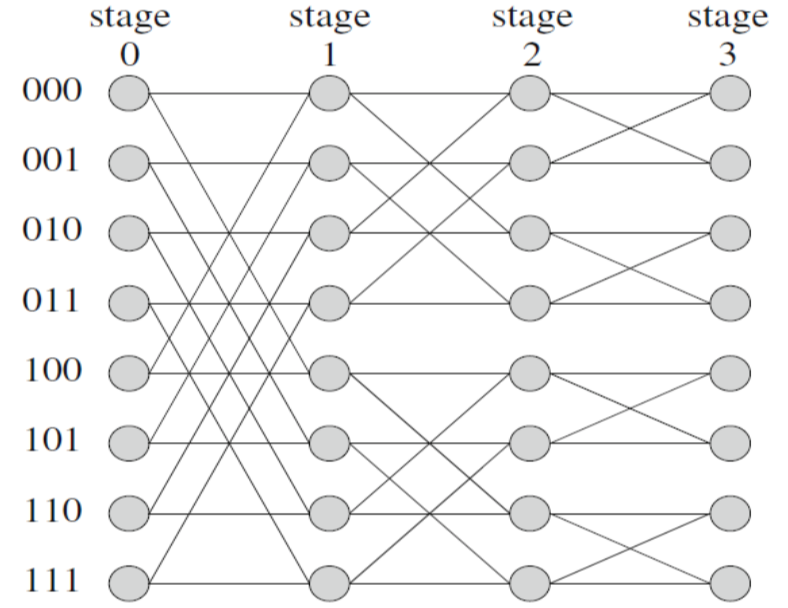
\includegraphics[width=\linewidth]{butterfly}
  \end{tabularx}
  \begin{tabularx}{0.32\linewidth}{X}
    Baseline \\
    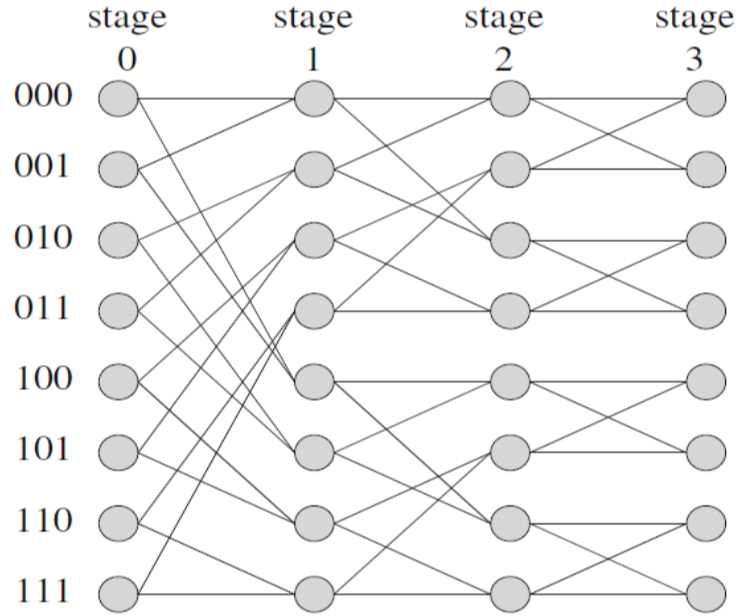
\includegraphics[width=\linewidth]{baseline}
  \end{tabularx}
  \subsection{Routing}
  Based on:
  \begin{itemize}
    \item Path length (minimal/non-minimal) whether shortest path
    \item Adaptivity (deterministic/adaptive) whether always the same path for same pair of nodes/take into account network status
  \end{itemize}
  3 deterministic examples
  \subsubsection{XY Routing for 2D Mesh}
  $(X_{src}, Y_{src})$ to $(X_{dst}, Y_{dst})$: move in x-direction until $X_{src} = X_{dst}$, then move in y-direction similarly
  \subsubsection{E-Cube Routing for Hypercube}
  No of bits difference b/w 2 pairs of nodes = number of hops (hamming distance). Start from MSB to LSB (or vice versa), find first different bit, go to the neighbouring node with the bit corrected.
  \subsubsection{XOR-Tag Routing for Omega Network}
  $T =$ Source Id $\oplus$ (XOR) Destination ID, at stage-$k$: go straight if bit $k$ of $T$ is $0$, crossover if bit $k$ of $T$ is $1$
\end{multicols*}
\end{document}
